The plots in F

\begin{figure}
  \centering
  \begin{subfigure}[b]{0.31\textwidth}
    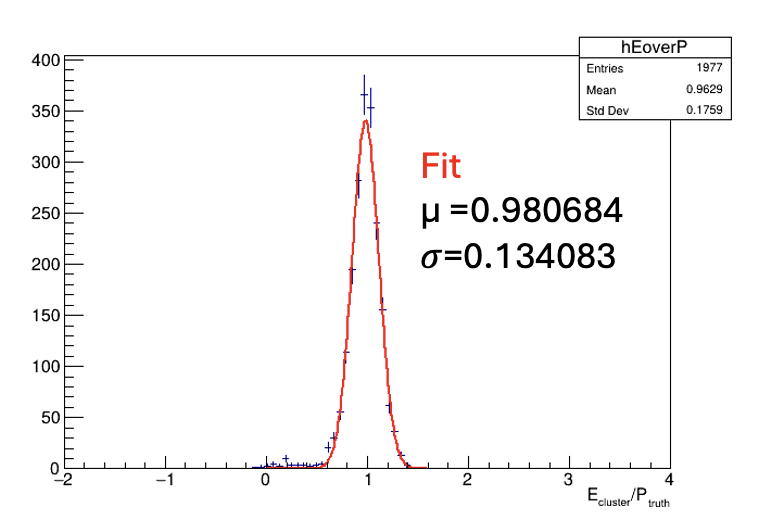
\includegraphics[width=\textwidth]{ueinpp/Figures/topocluster_noise/Resolution_topocluster/ep_2sigma.png}
    \caption{$2\sigma$}
  \end{subfigure}
  \hfill
  \begin{subfigure}[b]{0.32\textwidth}
    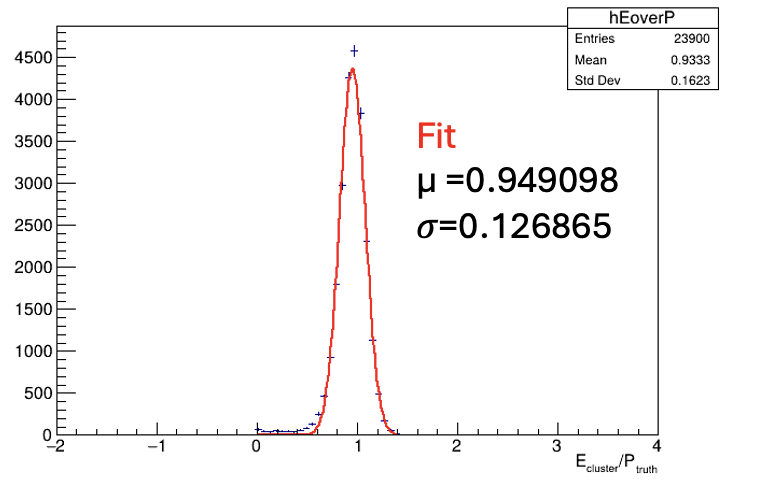
\includegraphics[width=\textwidth]{ueinpp/Figures/topocluster_noise/Resolution_topocluster/ep_3sigma.png}
    \caption{$3\sigma$}
  \end{subfigure}
  \hfill
  \begin{subfigure}[b]{0.31\textwidth}
    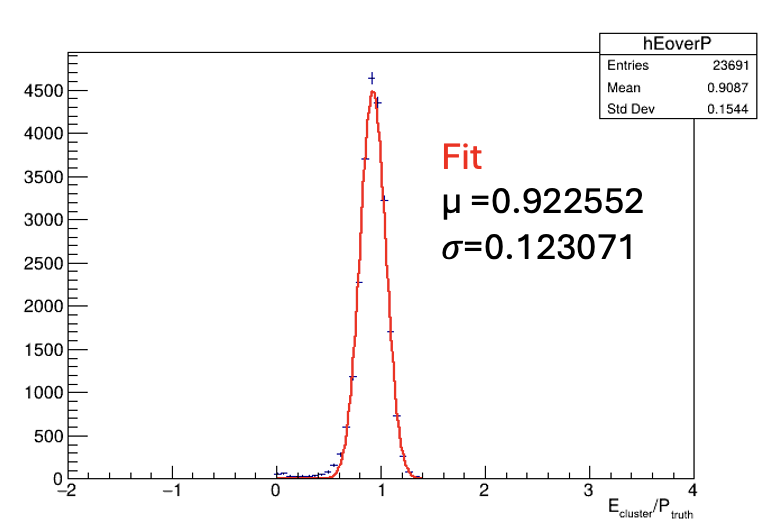
\includegraphics[width=\textwidth]{ueinpp/Figures/topocluster_noise/Resolution_topocluster/ep_4sigma.png}
    \caption{$4\sigma$}
  \end{subfigure}
  \caption{$E/P$ distributions for electromagnetic particles at $\Delta R < 0.1$ for different noise thresholds.}
  \label{fig:ep_resolution}
\end{figure}

\begin{figure}
  \centering
  \begin{subfigure}[b]{0.32\textwidth}
    \centering
    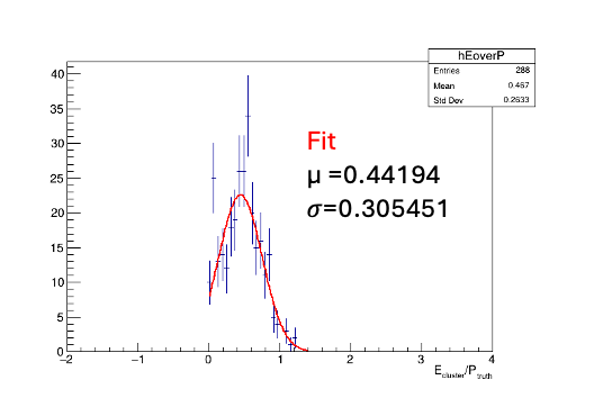
\includegraphics[width=\textwidth]{ueinpp/Figures/topocluster_noise/Resolution_topocluster/ep_hadronic_2sigma_e3gev_dr02.png}
    \caption{$2\sigma$}
  \end{subfigure}
  \hfill
  \begin{subfigure}[b]{0.32\textwidth}
    \centering
    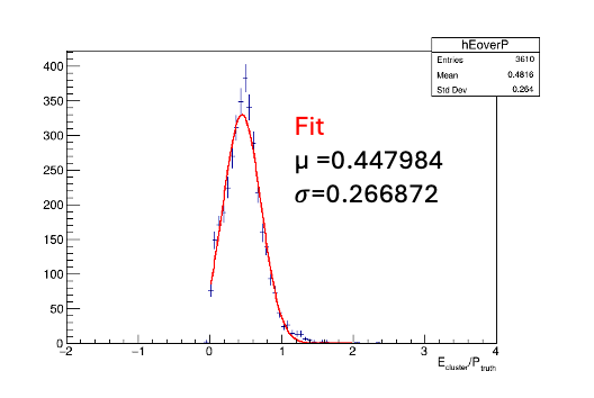
\includegraphics[width=\textwidth]{ueinpp/Figures/topocluster_noise/Resolution_topocluster/ep_hadronic_3sigma_e3gev_dr02.png}
    \caption{$3\sigma$}
  \end{subfigure}
  \hfill
  \begin{subfigure}[b]{0.32\textwidth}
    \centering
    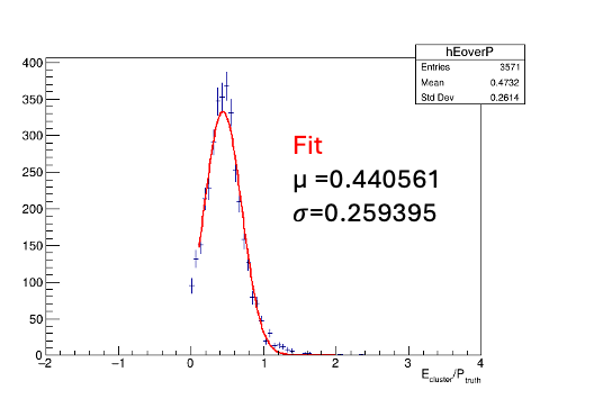
\includegraphics[width=\textwidth]{ueinpp/Figures/topocluster_noise/Resolution_topocluster/ep_hadronic_4sigma_e3gev_dr02.png}
    \caption{$4\sigma$}
  \end{subfigure}
  \caption{$E/P$ distributions for hadronic particles with $E > 3$\,GeV at $\Delta R < 0.2$ for different noise thresholds.}
  \label{fig:ep_hadronic_dr02_e3gev}
\end{figure}

The analysis below is an extension of the analysis outlined in Section~\ref{sec:topo_resolution} using $\Delta R < 0.1$ for the truth-cluster matching distance threshold and using track projections for track-cluster matching to further understand the topocluster resolution performance. For hadronic clusters, the resolution is studied under two energy selection criteria: $E > 1$\,GeV and $E > 3$\,GeV. 

\begin{figure}[h!]
  \centering

  \begin{subfigure}[t]{0.32\textwidth}
    \centering
    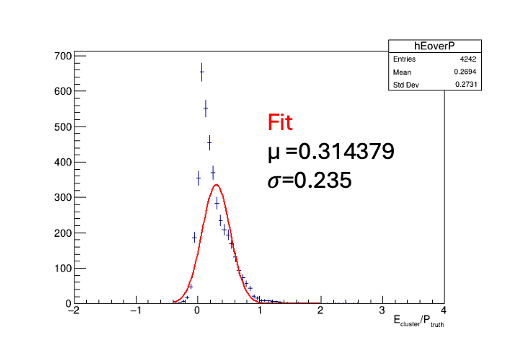
\includegraphics[width=\textwidth]{ueinpp/Figures/topocluster_noise/Resolution_topocluster/ep_hadronic_2sigma_e1gev_dr01.png}
    \caption{$2\sigma$}
  \end{subfigure}
  \hfill
  \begin{subfigure}[t]{0.32\textwidth}
    \centering
    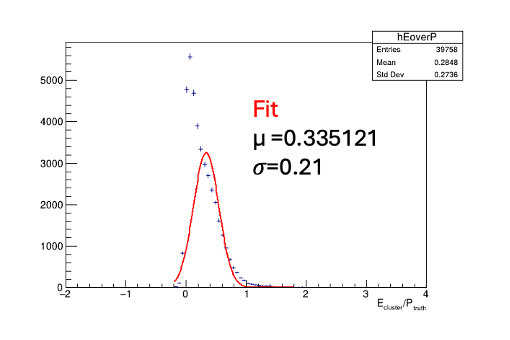
\includegraphics[width=\textwidth]{ueinpp/Figures/topocluster_noise/Resolution_topocluster/ep_hadronic_3sigma_e1gev_dr01.png}
    \caption{$3\sigma$}
  \end{subfigure}
  \hfill
  \begin{subfigure}[t]{0.32\textwidth}
    \centering
    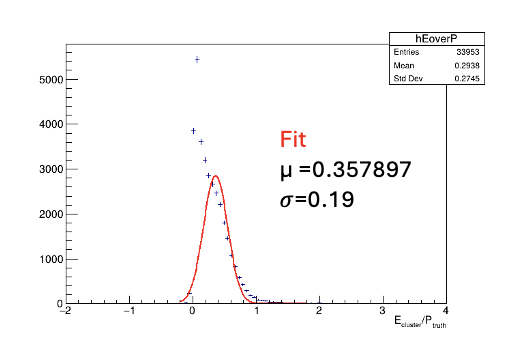
\includegraphics[width=\textwidth]{ueinpp/Figures/topocluster_noise/Resolution_topocluster/ep_hadronic_4sigma_e1gev_dr01.png}
    \caption{$4\sigma$}
  \end{subfigure}

  \caption{$E/P$ distributions for hadronic particles with $E > 1$\,GeV at $\Delta R < 0.1$ for different noise thresholds.}
  \label{fig:ep_hadronic_dr01_e1gev}
\end{figure}

\begin{figure}[h!]
  \centering
  \begin{subfigure}[t]{0.32\textwidth}
    \centering
    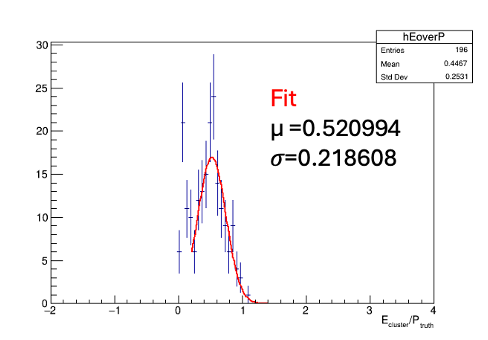
\includegraphics[width=\textwidth]{ueinpp/Figures/topocluster_noise/Resolution_topocluster/ep_hadronic_1sigma_e3gev_dr01.png}
    \caption{$1\sigma$}
  \end{subfigure}
  \hfill
  \begin{subfigure}[t]{0.325\textwidth}
    \centering
    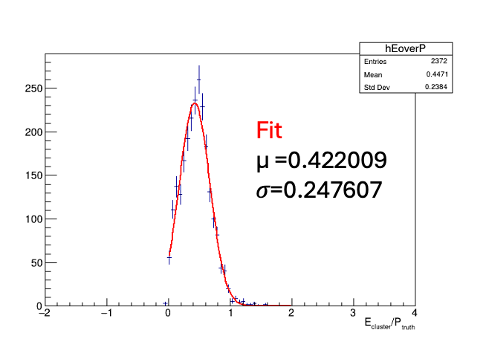
\includegraphics[width=\textwidth]{ueinpp/Figures/topocluster_noise/Resolution_topocluster/ep_hadronic_2sigma_e3gev_dr01.png}
    \caption{$2\sigma$}
  \end{subfigure}
  \hfill
  \begin{subfigure}[t]{0.305\textwidth}
    \centering
    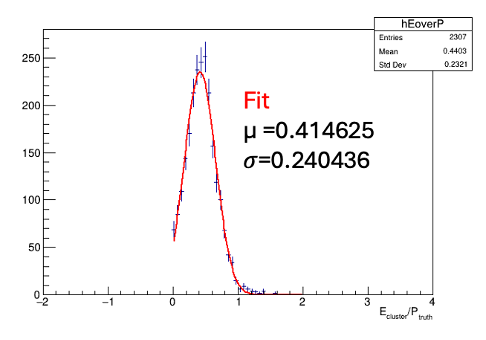
\includegraphics[width=\textwidth]{ueinpp/Figures/topocluster_noise/Resolution_topocluster/ep_hadronic_3sigma_e3gev_dr01.png}
    \caption{$3\sigma$}
  \end{subfigure}
  \caption{$E/P$ distributions for hadronic particles with $E > 3$\,GeV at $\Delta R < 0.1$ for different noise thresholds.}
  \label{fig:ep_hadronic_dr01_e3gev}
\end{figure}

The E/P distributions shown in Figure~\ref{fig:ep_hadronic_dr01_e1gev} for $\Delta R < 0.1$ and $E > 1$ GeV do not have a nice gaussian shape and instead look like they are being cut off at the low E/P range. This phenomena agrees with the physical understanding that this sample of hadrons is dominated by low $p_{T}$ hadrons which should have fairly large bending within the magnetic field. In our matching of truth particles to reconstructed clusters here we are not taking into account the bending from the magnetic field.

This theory can be first tested by using the same matching distance ($\Delta R < 0.1$), but with a higher energy threshold ($E > 3$\,GeV) where the hadrons should not be bent as much by the magnetic field. Here, the $E/P$ distributions are also studied for the $2\sigma$, $3\sigma$, and $4\sigma$ noise levels. The corresponding histograms are shown in Fig.~\ref{fig:ep_hadronic_dr01_e3gev}. These distributions are more gaussian and the distribution does not look like it is being cut off in the low E/P region like it did for the lower E hadrons.

The theory that the E/P distributions for low energy hadrons is being clipped geometrically can be further tested by using the track projection objects to the calorimeter faces to enhance our matching techniques. This study is performed using the $3\sigma$ noise threshold and selecting clusters with $E >$ 1 or 3 GeV. Two matching distances, $\Delta R < 0.1$ and $\Delta R < 0.2$, are considered. The applied tracking cuts include:  
\begin{itemize}
    \item an isolation requirement where no other truth particles with $p_T > 0.2$ GeV exist within $\Delta R < 0.6$ of the target track
    \item a transverse momentum threshold of either $p_T >$ 1 or 3 GeV for the truth particle
    \item a tighter vertex cut of $|z| < 10$ cm when using tracking information
\end{itemize}

These criteria aim to ensure clean and well-reconstructed matches between tracks and calorimeter clusters, providing a more accurate estimate of the topocluster energy resolution. The track projection algorithm included in the sPHENIX core software is used to find the track projection to the calorimeter layer faces. The projection to each of the calorimeter layer faces (EMCal, IHCal and OHCal) are included in this study. 
The $E/P$ distributions for tracks with $E > 1$\,GeV and track-cluster matching criteria of $\Delta R < 0.1$ and $\Delta R < 0.2$ intersecting the EMCal, IHCal, and OHCal front faces are shown in Figures~\ref{fig:ep_trackmatched_e1gev_dr01} and \ref{fig:ep_trackmatched_e1gev_dr02}, respectively.

\begin{figure}
  \centering
  \begin{subfigure}[b]{0.32\textwidth}
    \centering
    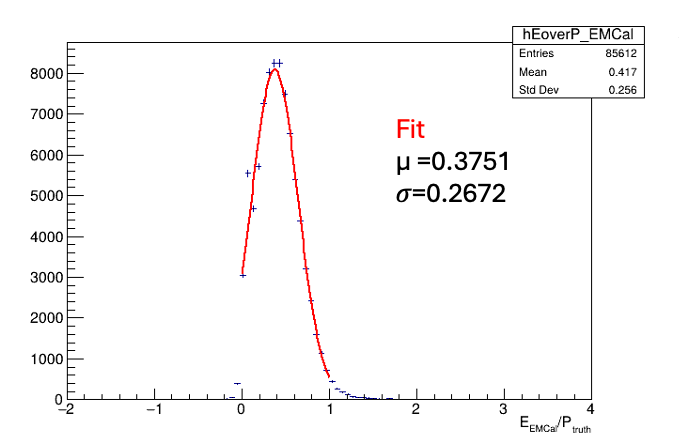
\includegraphics[width=\textwidth]{ueinpp/Figures/topocluster_noise/Resolution_topocluster/ep_trackmatched_emcal_e1gev_dr01.png}
    \caption{EMCal}
  \end{subfigure}
  \hfill
  \begin{subfigure}[b]{0.32\textwidth}
    \centering
    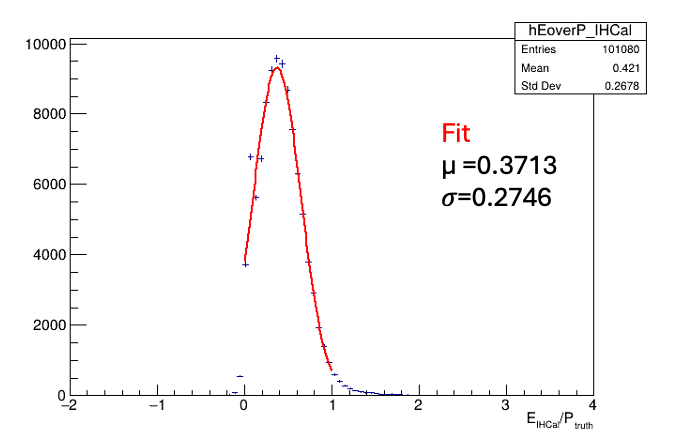
\includegraphics[width=\textwidth]{ueinpp/Figures/topocluster_noise/Resolution_topocluster/ep_trackmatched_ihcal_e1gev_dr01.png}
    \caption{IHCal}
  \end{subfigure}
  \hfill
  \begin{subfigure}[b]{0.32\textwidth}
    \centering
    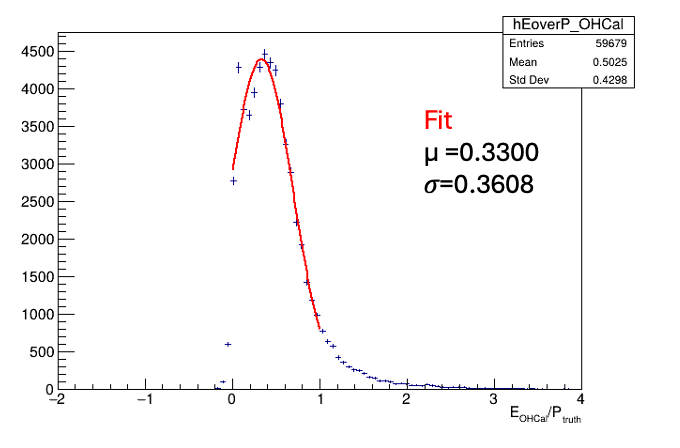
\includegraphics[width=\textwidth]{ueinpp/Figures/topocluster_noise/Resolution_topocluster/ep_trackmatched_ohcal_e1gev_dr01.png}
    \caption{OHCal}
  \end{subfigure}
  \caption{$E/P$ distributions for hadronic particles with $E > 1$\,GeV and $\Delta R < 0.1$, where the matched track has hits in the EMCal, IHCal, and OHCal calorimeter layers.}
  \label{fig:ep_trackmatched_e1gev_dr01}
\end{figure}

\begin{figure}
  \centering
  \begin{subfigure}[b]{0.32\textwidth}
    \centering
    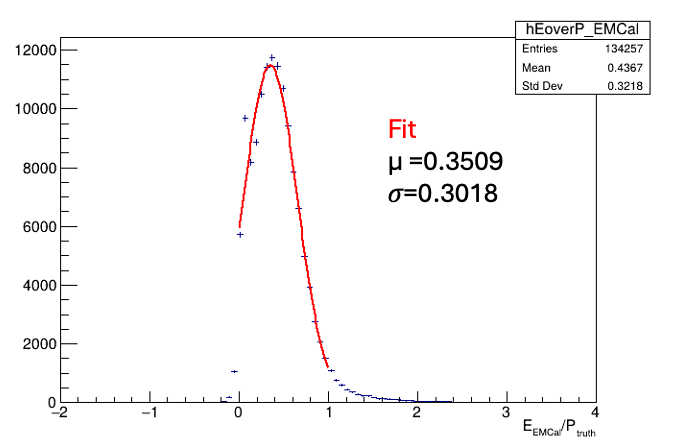
\includegraphics[width=\textwidth]{ueinpp/Figures/topocluster_noise/Resolution_topocluster/ep_trackmatched_emcal_e1gev_dr02.png}
    \caption{EMCal}
  \end{subfigure}
  \hfill
  \begin{subfigure}[b]{0.32\textwidth}
    \centering
    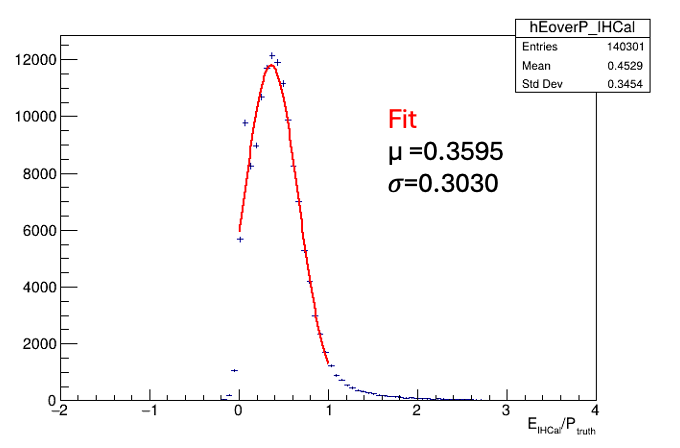
\includegraphics[width=\textwidth]{ueinpp/Figures/topocluster_noise/Resolution_topocluster/ep_trackmatched_ihcal_e1gev_dr02.png}
    \caption{IHCal}
  \end{subfigure}
  \hfill
  \begin{subfigure}[b]{0.32\textwidth}
    \centering
    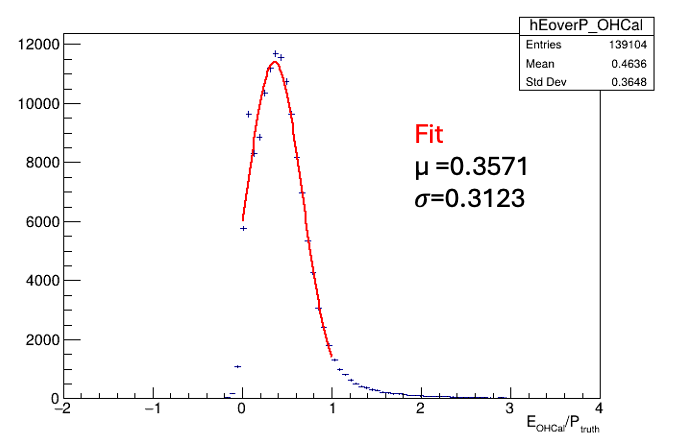
\includegraphics[width=\textwidth]{ueinpp/Figures/topocluster_noise/Resolution_topocluster/ep_trackmatched_ohcal_e1gev_dr02.png}
    \caption{OHCal}
  \end{subfigure}
  \caption{$E/P$ distributions for hadronic particles with $E > 1$\,GeV and $\Delta R < 0.2$, where the matched track has hits in the EMCal, IHCal, and OHCal calorimeter layers.}
  \label{fig:ep_trackmatched_e1gev_dr02}
\end{figure}

In both the $\Delta R < 0.1$ and $\Delta R < 0.2$ cases the E/P distribution when include track projection in the track-cluster matching gives a much more gaussian distribution and the clipped distribution effect seen for low E hadrons in the more basic truth particle to cluster matching is no longer present. 
Therefore, it can be understood that for low energy hadrons ($\sim 1$ GeV) including the projection to the calorimeter face is important in matching of tracks/truth particles to calorimeter clusters.
Also it is notable from Figures~\ref{fig:ep_trackmatched_e1gev_dr01} and \ref{fig:ep_trackmatched_e1gev_dr02} that the projections that produce the best matching are to the EMCal or IHCal front face. The OHCal front face produces a wider E/P distribution with a larger fraction of clipped parts of the distribution.
